\subsection{Period 3: Absence of the DHL, with sporadic transitory layers after the Northern Spring Equinox (2012-2015) - $L_s=\ang{30}-\ang{75}$}

During this period (Fig.~\ref{fig:dhl_2012_2015}), the main haze layer has large-scale structures which slowly evolve under the influence of the
large-scale circulation. The south and north polar hoods are still visible and they evolve
with time. Superimposed on this background haze, transient structures show up and disappear from one observation
to the other. At some moments, large-scale detached hazes appear. They differ from the detached haze seen at the
beginning of the mission because they are not stable in time and in altitude.

\begin{figure*}[!ht]
\plotone{Fig/Lat_beta-2012_2015}
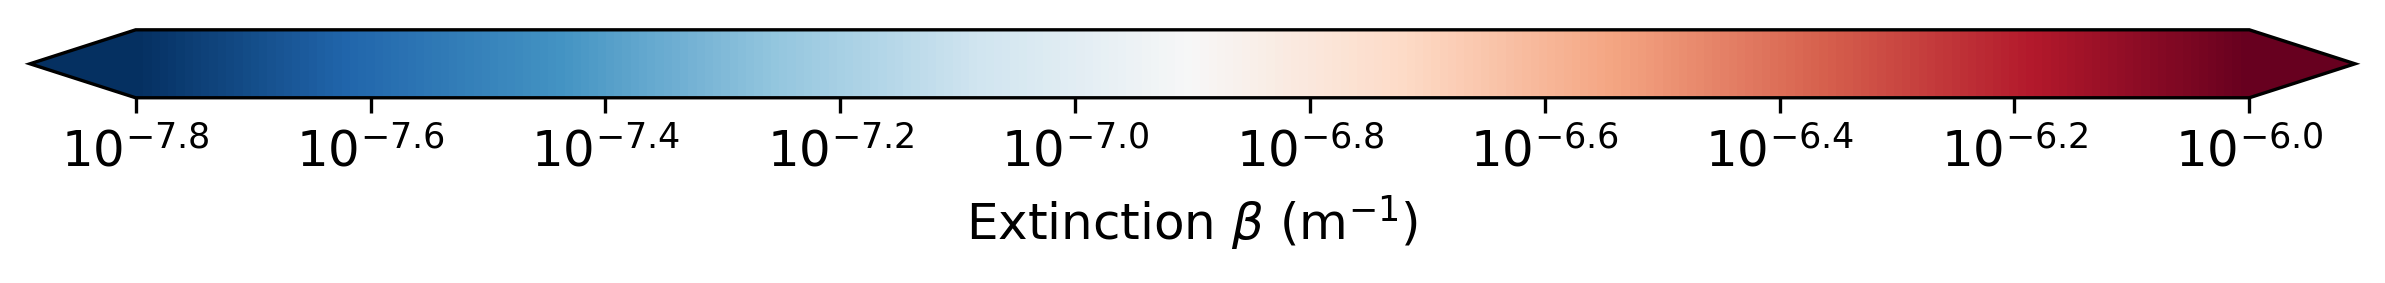
\includegraphics[width=.5\textwidth]{Fig/Extinction_colorbar}
\caption{Same as the figures~\ref{fig:dhl_2004_2008} and~\ref{fig:dhl_2008_2012}
for 4 images taken between 2012 and 2015 ($L_s=\ang{30}-\ang{75}$) showing sporadic
transitory layers and the absence of a stable DHL.
The color scheme is the same as in previous figures and the altitude extends down to 350 km.}
\label{fig:dhl_2012_2015}
\end{figure*}

In April 2012 (Fig.~\ref{fig:dhl_2012_2015}a), the detached haze has completely disappeared, except some residual
structures around the equator at 370 km.
These relics of the last detached haze layer are almost not perceptible in the corresponding I/F profile. At other
latitudes, we can see only the main haze with a marked south polar hood and a small increase of extinction above
\ang{65}N that could be the residual north polar hood. Sometimes, detached layers emerge from the background with large latitudinal
extent (e.g. detached haze at 500 km Fig.~\ref{fig:dhl_2012_2015}b). However, they only remain for a short time
and are not seen in the following observations.

In August 2014 (Fig.~\ref{fig:dhl_2012_2015}c) we observed a plume of aerosol between \ang{10}S and \ang{25}N,
reaching 530 km. A detached haze layer seems to spread from this plume toward the north and the south. This
detached haze is around 500 km altitude, descending to 470 km at \ang{50}S (and probably even further south). In the
north, the detached haze does not extend further than \ang{50}N and remains at 500 km. This indicates an
atmosphere circulation flowing from equator toward the south pole. These aerosols seem to originate
from the equatorial part of the main haze.

Most of the observations between 2012 and the end of 2015 are featureless as in figure~\ref{fig:dhl_2012_2015}d)
taken in October, 2015. During this period, the main haze has a uniform scale height of 45 km and
with an homogeneous extinction at the planetary scale.
